\subsection{Neural networks}

Neural networks (NNs) are an immensely rich and complicated topic. In this chapter, we introduce the simple ideas and concepts behind the most simple architectures of NNs. For more exhaustive treatments on NN idiosyncracies, we refer to the monographs by \cite{haykin2009neural}, \cite{du2013neural} and \cite{goodfellow2016deep}. The latter is available freely online: \href{http://www.deeplearningbook.org}{www.deeplearningbook.org}. For a practical introduction, we recommend the great book of \cite{chollet2017deep}.

For starters, we briefly comment on the qualification ``neural network''. Most experts agree that the term is not very well chosen, as NNs have little to do with how the human brain works (of which we know not that much). This explains why they are often referred to as ``artificial neural networks'' - we do not use the adjective for notational simplicity. Because we consider it more appropriate, we recall the definition of NNs given by François Chollet: ``\textit{chains of differentiable, parameterised geometric functions, trained with gradient descent (with gradients obtained via the chain rule)}''.

Early references of neural networks in finance are \cite{bansal1993no} and \cite{eakins1998analyzing}. Both have very different goals. In the first one, the authors aim to estimate a \textbf{nonlinear form} for the pricing kernel. In the second one, the purpose is to identify and quantify relationships between institutional investments in stocks and the attributes of the firms (an early contribution towards factor investing). An early review \citep{burrell1997impact} lists financial applications of NNs during the 1990s. More recently, \cite{sezer2019financial}, \cite{jiang2020applications} and \cite{lim2020time} survey the attempts to forecast financial time series with deep-learning models, mainly by computer science scholars.

\subsubsection{The original perceptron}

The origins of NNs go back at least to \cite{rosenblatt1958perceptron}. Its aim is binary classification. For simplicity, let us assume that the output is $\{0$ = do not invest$\}$ versus $\{1$ = invest$\}$ (e.g., derived from return, negative versus positive). Given the current nomenclature, a perceptron can be defined as an activated linear mapping. The model is the following:

\begin{equation}
f(\mathbf{x})=\left\{ \begin{array}{lll}
1 & \text{if } \mathbf{x}'\mathbf{w}+b >0\\
0  &\text{otherwise}
\end{array}\right.
\end{equation}

The vector of weights $\mathbf{w}$ scales the variables and the bias $b$ shifts the decision barrier.

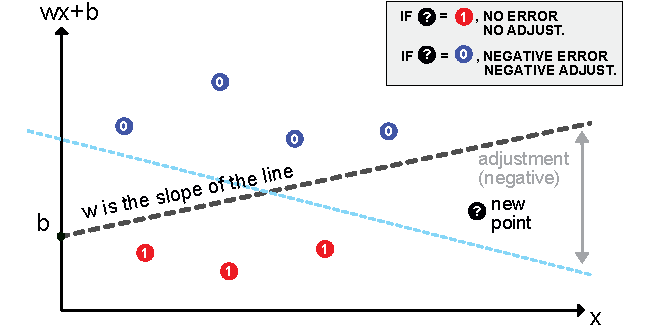
\includegraphics[width=0.7\linewidth]{files/NN_percep_scheme-0f68ea3e26672006d3f08b7ad43f9b31.pdf}

\subsubsection{Multilayer perceptron}

\paragraph{Introduction and notations}

A perceptron can be viewed as a linear model to which is applied a particular function: the Heaviside (step) function. Other choices of functions are naturally possible. In the NN jargon, they are called activation functions. Their purpose is to introduce nonlinearity in otherwise very linear models.

Just like for random forests with trees, the idea behind neural networks is to combine perceptron-like building blocks.

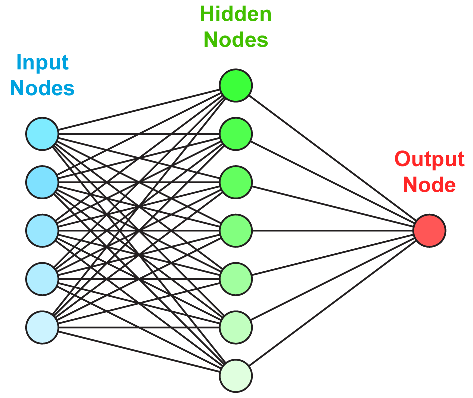
\includegraphics[width=0.7\linewidth]{files/nn-a2dde54f7cb0c2b9c548a1323f3b25c8.pdf}

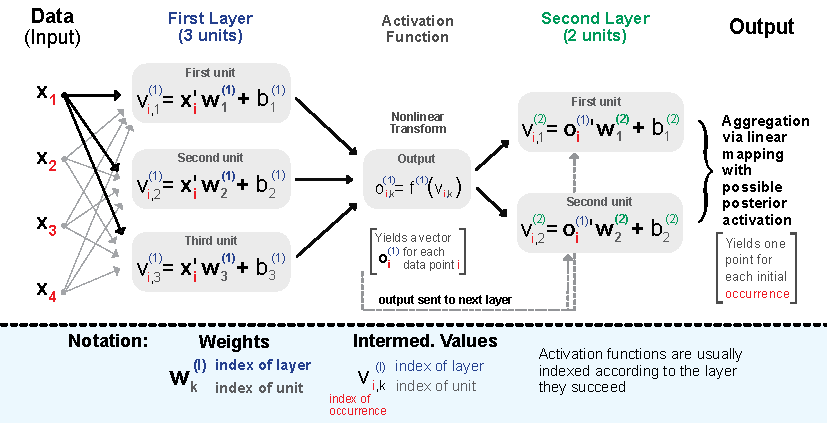
\includegraphics[width=0.7\linewidth]{files/NN_scheme-ac4550766019d6a831579fbda63be208.pdf}

The process is the following. When entering the network, the data goes though the initial linear mapping:\newline
\begin{equation}
v_{i,k}^{(1)}=\textbf{x}_i'\textbf{w}^{(1)}_k+b_k^{(1)},  \text{for } l=1, \quad k \in [1,U_1],
\end{equation}
\newline
which is then transformed by a non-linear function $f^{1}$.

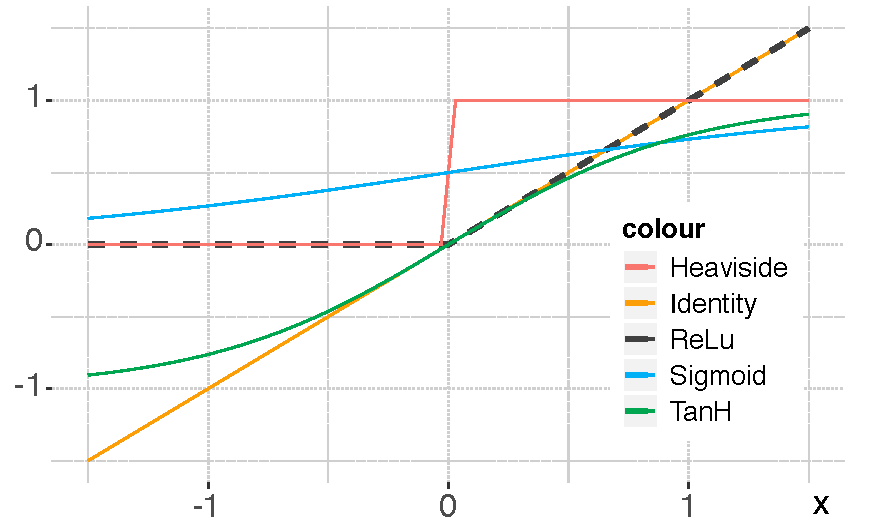
\includegraphics[width=0.7\linewidth]{files/activation-ce4d0d01bdbe93148a34dd7831f38a1e.pdf}

\paragraph{Universal approximation}

One reason neural networks work well is that they are \textit{universal approximators}. Given any bounded continuous function, there exists a one-layer network that can approximate this function up to arbitrary precision.

\begin{equation}
\mathbb{E}\left[(f(x)-f_n(x))^2 \right]=\underbrace{O\left(\frac{c_f}{n} \right)}_{\text{size of network}}+\ \underbrace{O\left(\frac{nK \log(N)}{N} \right)}_{\text{size of sample}},
\end{equation}

\paragraph{Learning via back-propagation}\label{backprop}

Just like for tree methods, neural networks are trained by minimizing some loss function subject to some penalization:
\begin{equation}
O=\sum_{i=1}^I \text{loss}(y_i,\tilde{y}_i)+ \text{penalization},
\end{equation}

The updating of the weights will be performed via gradient descent:

\begin{equation}
\textbf{W} \leftarrow \textbf{W}-\eta  \frac{\partial D(\tilde{y}_i) }{\partial \textbf{W}}.
\end{equation}

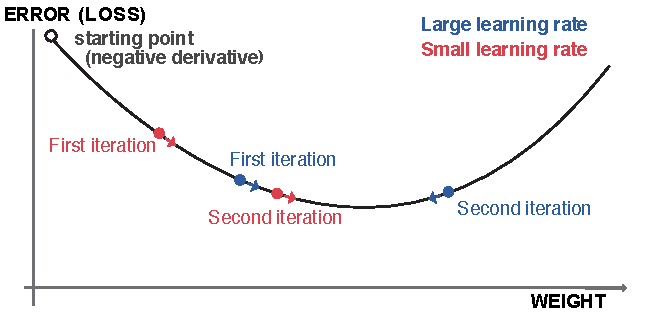
\includegraphics[width=0.7\linewidth]{files/Newton-f185a77ed7d0bde9f6bd8f5d61721a2f.pdf}

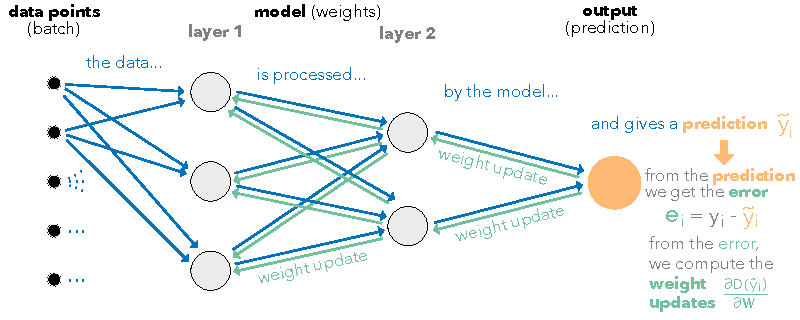
\includegraphics[width=0.7\linewidth]{files/backprop-910104d5ca67cadfed531a35130ca7bc.pdf}

\paragraph{Further details on classification}\label{NNclass}

Facing a classification problem, the trick is to use an appropriate activation function at the very end of the network. The most commonly used activation is the so-called \textit{softmax} function:

\begin{equation}
\tilde{\textbf{y}}_i=s(\textbf{x})_i=\frac{e^{x_i}}{\sum_{j=1}^Je^{x_j}}.
\end{equation}

The cross-entropy is defined as:

\begin{equation}
\text{CE}(\textbf{y}_i,\tilde{\textbf{y}}_i)=-\sum_{j=1}^J\log(\tilde{y}_{i,j})y_{i,j}.
\end{equation}

\subsubsection{How deep we should go and other practical issues}\label{howdeep}

\paragraph{Architectural choices}

The number of hidden layers in current financial applications rarely exceeds three or four. The number of units per layer $(U_k)$ is often chosen to follow the geometric pyramid rule:
\begin{equation}
U_k\approx \left\lfloor O\left( \frac{I}{O}\right)^{\frac{L+1-k}{L+1}}\right\rfloor.
\end{equation}

\paragraph{Penalizations and dropout}

\begin{equation}
O=\sum_{i=1}^I \text{loss}(y_i,\tilde{y}_i)+ \sum_{k} \lambda_k||\textbf{W}_k||_1+ \sum_j\delta_j||\textbf{W}_j||_2^2,
\end{equation}

\subsubsection{Code samples and comments for vanilla MLP}

\paragraph{Regression example}

Before we head to the core of the NN, a short stage of data preparation is required.

\begin{verbatim}
import numpy as np
import pandas as pd
import matplotlib.pyplot as plt
import warnings
warnings.filterwarnings('ignore')
plt.style.use('seaborn-v0_8-whitegrid')
\end{verbatim}

\begin{verbatim}
import os
os.environ["KERAS_BACKEND"] = "jax"  # or "torch"

import keras
from keras import layers
\end{verbatim}

\begin{verbatim}
from keras import layers, regularizers, constraints, initializers, callbacks

from data_build import generate_data
data_ml, features, features_short, returns, stock_ids, stock_ids_short = generate_data()
features_short =["Div_yld", "EPS", "size_avg_252d", "mom_252", "OCF_Growth_1Y", "PB", "vol_252"]
separation_date = "2017-01-15"

# Data preparation
data_ml_clean = data_ml.dropna()
training_sample = data_ml_clean[data_ml['date'] <= separation_date]
testing_sample = data_ml_clean[data_ml['date'] > separation_date] 
NN_train_features = training_sample[features].values    # Training features
NN_train_labels = training_sample['R1M'].values         # Training labels
NN_test_features = testing_sample[features].values      # Testing features
NN_test_labels = testing_sample['R1M'].values           # Testing labels
\end{verbatim}

In Keras, the training of neural networks is performed through three steps: defining the structure, setting the loss function, and training.

\begin{verbatim}
# Define the structure of the network
model = keras.Sequential([
    layers.Dense(units=16, activation='relu', input_shape=(NN_train_features.shape[1],)),
    layers.Dense(units=8, activation='tanh'),
    layers.Dense(units=1)  # No activation means linear activation: f(x) = x
])
\end{verbatim}

\begin{verbatim}
# Model specification
model.compile(
    loss='mean_squared_error',
    optimizer='rmsprop',
    metrics=['mean_absolute_error']
)
model.summary()
\end{verbatim}

\begin{verbatim}
Model: "sequential"
\end{verbatim}

\begin{verbatim}
+---------------------------------+------------------------+---------------+
| Layer (type)                    | Output Shape           |       Param # |
+---------------------------------+------------------------+---------------+
| dense (Dense)                   | (None, 16)             |         1,968 |
+---------------------------------+------------------------+---------------+
| dense_1 (Dense)                 | (None, 8)              |           136 |
+---------------------------------+------------------------+---------------+
| dense_2 (Dense)                 | (None, 1)              |             9 |
+---------------------------------+------------------------+---------------+
\end{verbatim}

\begin{verbatim}
Total params: 2,113 (8.25 KB)
\end{verbatim}

\begin{verbatim}
Trainable params: 2,113 (8.25 KB)
\end{verbatim}

\begin{verbatim}
Non -trainable params: 0 (0.00 B)
\end{verbatim}

\begin{verbatim}
# Train the model
history = model.fit(
    NN_train_features, NN_train_labels,
    epochs=10, batch_size=512,
    validation_data=(NN_test_features, NN_test_labels)
)

# Plot training history
fig, axes = plt.subplots(1, 2, figsize=(12, 4))
axes[0].plot(history.history['loss'], label='Training')
axes[0].plot(history.history['val_loss'], label='Validation')
axes[0].set_xlabel('Epoch'); axes[0].set_ylabel('Loss'); axes[0].legend()
axes[1].plot(history.history['mean_absolute_error'], label='Training')
axes[1].plot(history.history['val_mean_absolute_error'], label='Validation')
axes[1].set_xlabel('Epoch'); axes[1].set_ylabel('MAE'); axes[1].legend()
plt.tight_layout(); plt.show()
\end{verbatim}

\begin{verbatim}
447/447 -------------------- 1s 1ms/step - loss: 5.6226e-04 - mean_absolute_error: 0.0211 - val_loss: 4.0773e-04 - val_mean_absolute_error: 0.0170
\end{verbatim}

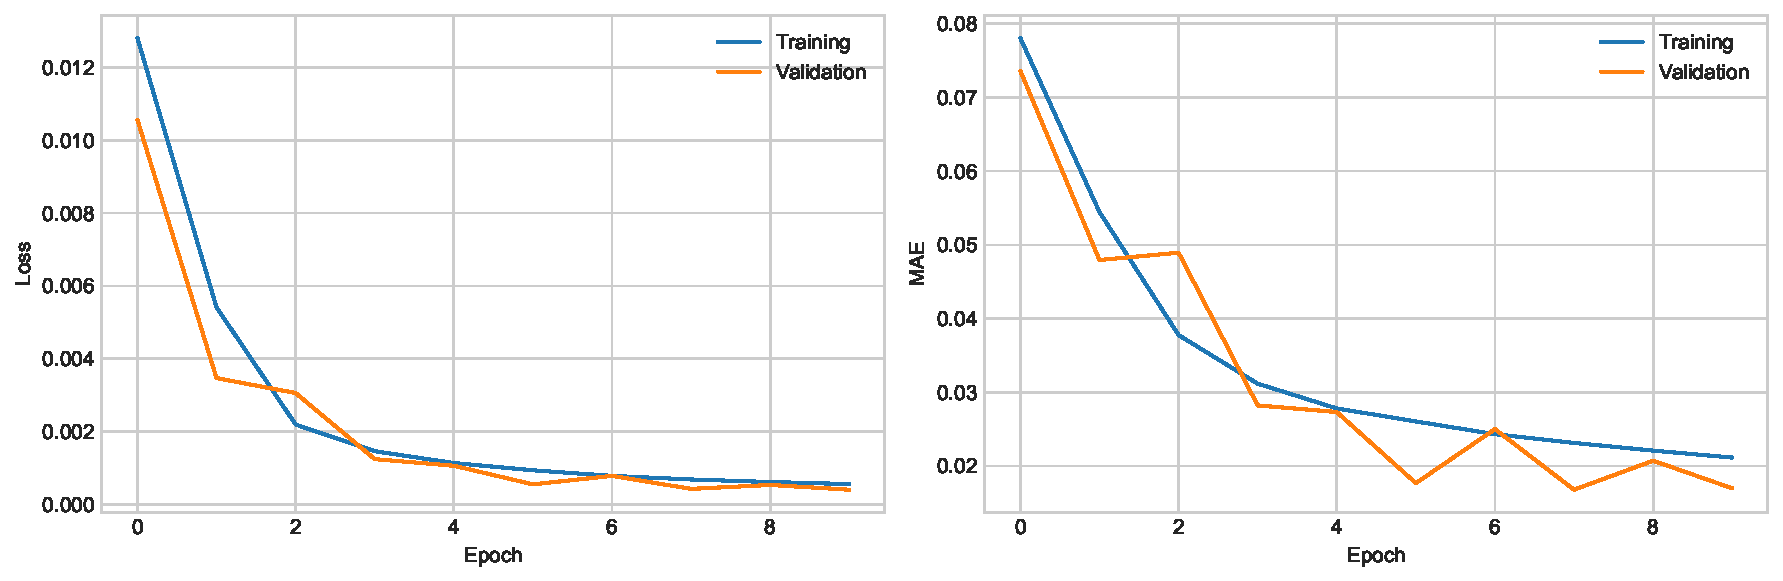
\includegraphics[width=0.7\linewidth]{files/5929b3f3ca8e2c9e99c5ade01646d8a0.pdf}

\begin{verbatim}
# Predictions and hit ratio
predictions = model.predict(NN_test_features).flatten()
hit_ratio = np.mean(predictions * NN_test_labels > 0)
print(f"Hit ratio: {np.round(hit_ratio, 5)}")
\end{verbatim}

\begin{verbatim}
4266/4266 -------------------- 1s 167us/step
\end{verbatim}

\begin{verbatim}
Hit ratio: 0.92084
\end{verbatim}

\paragraph{Classification example}

We pursue our exploration of neural networks with a classification task on the binary label R1M\_C.

\begin{verbatim}
# One-hot encoding of the labels
NN_train_labels_C = pd.get_dummies(training_sample['R1M_C']).values
NN_test_labels_C = pd.get_dummies(testing_sample['R1M_C']).values
\end{verbatim}

\begin{verbatim}
# Define the structure with additional features
model_C = keras.Sequential([
    layers.Dense(units=16, activation='tanh',
                 input_shape=(NN_train_features.shape[1],),
                 kernel_initializer='random_normal',
                 kernel_constraint=constraints.NonNeg()),
    layers.Dropout(rate=0.25),
    layers.Dense(units=8, activation='elu',
                 bias_initializer=initializers.Constant(0.2),
                 kernel_regularizer=regularizers.l2(0.01)),
    layers.Dense(units=2, activation='softmax')
])
\end{verbatim}

\begin{verbatim}
# Model specification
model_C.compile(
    loss='binary_crossentropy',
    optimizer=keras.optimizers.Adam(learning_rate=0.005, beta_1=0.9, beta_2=0.95),
    metrics=['categorical_accuracy']
)
model_C.summary()
\end{verbatim}

\begin{verbatim}
Model: "sequential_1"
\end{verbatim}

\begin{verbatim}
+---------------------------------+------------------------+---------------+
| Layer (type)                    | Output Shape           |       Param # |
+---------------------------------+------------------------+---------------+
| dense_3 (Dense)                 | (None, 16)             |         1,968 |
+---------------------------------+------------------------+---------------+
| dropout (Dropout)               | (None, 16)             |             0 |
+---------------------------------+------------------------+---------------+
| dense_4 (Dense)                 | (None, 8)              |           136 |
+---------------------------------+------------------------+---------------+
| dense_5 (Dense)                 | (None, 2)              |            18 |
+---------------------------------+------------------------+---------------+
\end{verbatim}

\begin{verbatim}
Total params: 2,122 (8.29 KB)
\end{verbatim}

\begin{verbatim}
Trainable params: 2,122 (8.29 KB)
\end{verbatim}

\begin{verbatim}
Non -trainable params: 0 (0.00 B)
\end{verbatim}

\begin{verbatim}
# Train with early stopping
early_stop = callbacks.EarlyStopping(monitor='val_loss', min_delta=0.001, patience=3, verbose=0)

history_C = model_C.fit(
    NN_train_features, NN_train_labels_C,
    epochs=20, batch_size=512,
    validation_data=(NN_test_features, NN_test_labels_C),
    verbose=0, callbacks=[early_stop]
)

# Plot
fig, axes = plt.subplots(1, 2, figsize=(12, 4))
axes[0].plot(history_C.history['loss'], label='Training')
axes[0].plot(history_C.history['val_loss'], label='Validation')
axes[0].set_xlabel('Epoch'); axes[0].set_ylabel('Loss'); axes[0].legend()
axes[1].plot(history_C.history['categorical_accuracy'], label='Training')
axes[1].plot(history_C.history['val_categorical_accuracy'], label='Validation')
axes[1].set_xlabel('Epoch'); axes[1].set_ylabel('Accuracy'); axes[1].legend()
plt.tight_layout(); plt.show()
\end{verbatim}

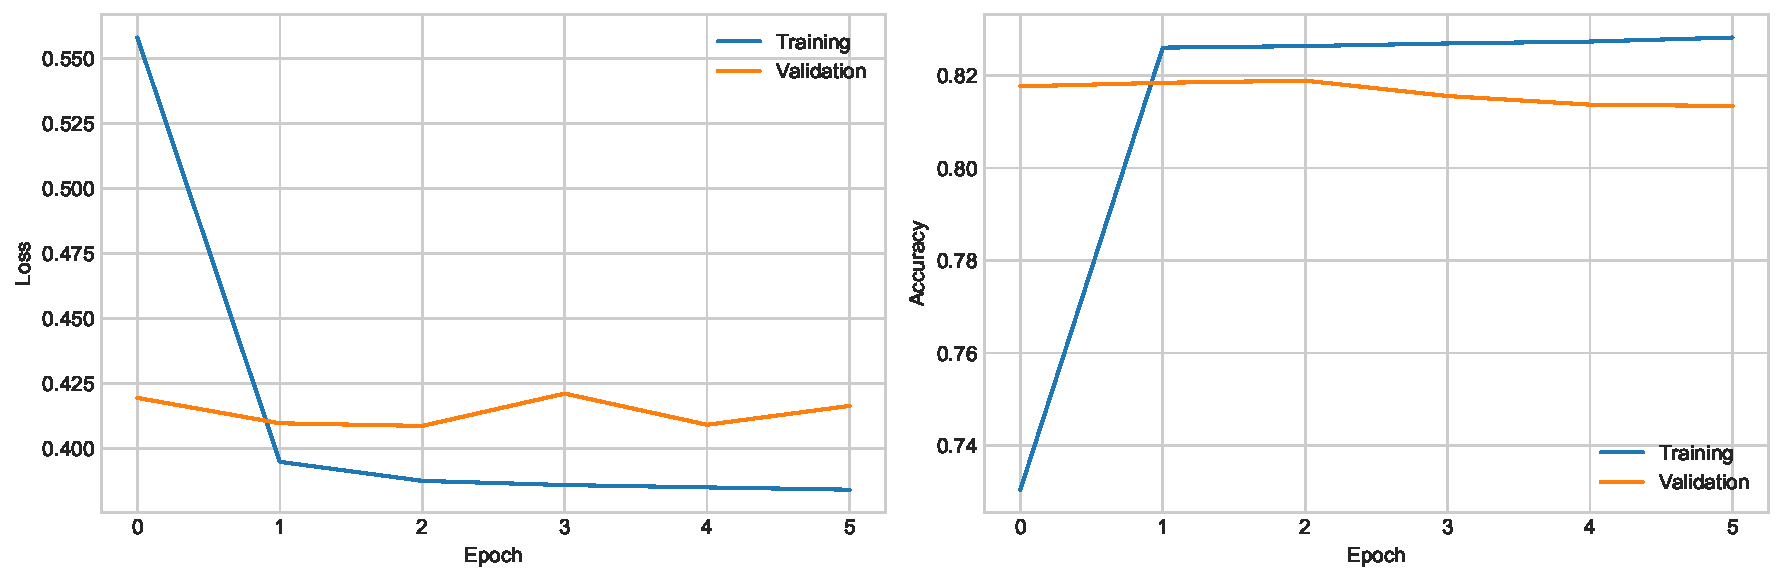
\includegraphics[width=0.7\linewidth]{files/d5aca84fc56e33c0829d122e108a4aa2.pdf}

\paragraph{Custom losses}\label{custloss}

In Keras, it is possible to define user-specified loss functions.

\begin{verbatim}
import keras.ops as ops

def custom_loss(y_true, y_pred):
    var_pred = ops.mean((y_pred - ops.mean(y_pred)) * (y_pred - ops.mean(y_pred)))
    cov_term = ops.mean((y_true - ops.mean(y_true)) * (y_pred - ops.mean(y_pred)))
    return var_pred - 5 * cov_term

model_custom = keras.Sequential([
    layers.Dense(units=16, activation='relu', input_shape=(NN_train_features.shape[1],)),
    layers.Dense(units=8, activation='sigmoid'),
    layers.Dense(units=1)
])

model_custom.compile(loss=custom_loss, optimizer='rmsprop', metrics=['mean_absolute_error'])
\end{verbatim}

\begin{verbatim}
# Train and evaluate
history_custom = model_custom.fit(
    NN_train_features, NN_train_labels,
    epochs=10, batch_size=512,
    validation_data=(NN_test_features, NN_test_labels)
)

predictions_custom = model_custom.predict(NN_test_features).flatten()
hit_ratio_custom = np.mean(predictions_custom * NN_test_labels > 0)
print(f"Hit ratio: {hit_ratio_custom}")
\end{verbatim}

\begin{verbatim}
4266/4266 -------------------- 1s 159us/step
\end{verbatim}

\begin{verbatim}
Hit ratio: 0.5995076995208861
\end{verbatim}

\subsubsection{Recurrent networks}\label{RNN}

\paragraph{Presentation}

Multilayer perceptrons are feed-forward networks because the data flows from left to right with no looping in between. For some particular tasks with sequential linkages, it might be useful to keep track of what happened with the previous sample.

\begin{equation}
\begin{aligned}
\tilde{y}_i&=f^{(y)}\left(\sum_{j=1}^{U_1}h_{i,j}w^{(y)}_j+b^{(2)}\right) \\
\textbf{h}_{i} &=f^{(h)}\left(\sum_{k=1}^{U_0}x_{i,k}w^{(h,1)}_k+b^{(1)}+ \underbrace{\sum_{k=1}^{U_1}  w^{(h,2)}_{k}h_{i-1,k}}_{\text{memory part}} \right),
\end{aligned}
\end{equation}

For a recent theoretical treatment, \cite{chen2026recurrent} derive statistical guarantees for recurrent networks under a broad class of nonlinear autoregressive processes with exogenous variables. They show that recurrence lets the network summarize the past through a compact hidden state instead of many explicit lags, which speeds up estimation compared to standard nonparametric regression.

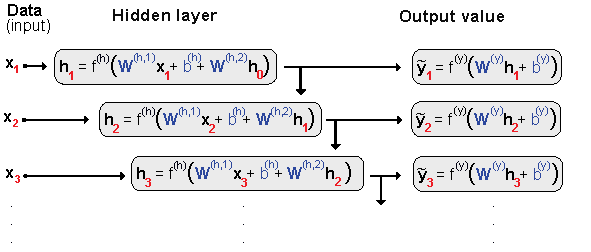
\includegraphics[width=0.7\linewidth]{files/RN-949eb92349432c0d079d12ac88f01871.pdf}

The Gated Recurrent Unit (GRU) has the following representation:
\begin{equation}
\begin{aligned}
\tilde{y}_i&=z_i\tilde{y}_{i-1}+ (1-z_i)\tanh \left(\textbf{w}_y'\textbf{x}_i+ b_y+ u_yr_i\tilde{y}_{i-1}\right) \\
z_i &= \text{sig}(\textbf{w}_z'\textbf{x}_i+b_z+u_z\tilde{y}_{i-1}) \\
r_i &= \text{sig}(\textbf{w}_r'\textbf{x}_i+b_r+u_r\tilde{y}_{i-1})
\end{aligned}
\end{equation}

\paragraph{Code and results}

\begin{verbatim}
# Dedicated dataset for RNN
data_rnn = data_ml[data_ml['fsym_id'].isin(stock_ids_short)]
training_sample_rnn = data_rnn[data_rnn['date'] < separation_date]
testing_sample_rnn = data_rnn[data_rnn['date'] > separation_date]

nb_stocks = len(stock_ids_short)
nb_feats = len(features)
nb_dates_train = len(training_sample_rnn) // nb_stocks
nb_dates_test = len(testing_sample_rnn) // nb_stocks
\end{verbatim}

\begin{verbatim}
# Format the data into arrays: (stock, date, feature)
train_features_rnn = training_sample_rnn[features].values.reshape(nb_stocks, nb_dates_train, nb_feats)
test_features_rnn = testing_sample_rnn[features].values.reshape(nb_stocks, nb_dates_test, nb_feats)
train_labels_rnn = training_sample_rnn['R1M'].values.reshape(nb_stocks, nb_dates_train, 1)
test_labels_rnn = testing_sample_rnn['R1M'].values.reshape(nb_stocks, nb_dates_test, 1)
\end{verbatim}

\begin{verbatim}
# Define the RNN model
model_RNN = keras.Sequential([
    layers.GRU(units=16, 
               #input_batch_size=nb_stocks,
               #input_shape=(nb_dates_train, nb_feats),
               activation='tanh', return_sequences=True),
    layers.Dense(units=1)
])

model_RNN.compile(loss='mean_squared_error', optimizer='rmsprop', metrics=['mean_absolute_error'])
\end{verbatim}

\begin{verbatim}
# Train the RNN model
history_RNN = model_RNN.fit(
    train_features_rnn, train_labels_rnn,
    epochs=10, batch_size=nb_stocks, verbose=0
)
\end{verbatim}

\begin{verbatim}
pred_rnn = model_RNN.predict(test_features_rnn, batch_size=nb_stocks)
hit_ratio_rnn = np.mean(pred_rnn.flatten() * test_labels_rnn.flatten() > 0)
print(f"Hit ratio: {hit_ratio_rnn}")
\end{verbatim}

\begin{verbatim}
1/1 -------------------- 0s 140ms/step
\end{verbatim}

\begin{verbatim}
Hit ratio: 0.4964004687761594
\end{verbatim}

\subsubsection{Other common architectures}

\paragraph{Generative adversarial networks}\label{generative-aversarial-networks}

GANs consist in two neural networks: the first one tries to learn and the second one tries to fool the first. $D$ and $G$ play the following minimax game:
\begin{equation}
\underset{G}{\min} \ \underset{D}{\max} \ \left\{ \mathbb{E}[\log(D(\textbf{x}))]+\mathbb{E}[\log(1-D(G(\textbf{z})))] \right\}.
\end{equation}

\paragraph{Autoencoders}\label{autoencoders}

AEs are a family of neural networks where the label is equal to the input:
\begin{equation}
\begin{array}{ccccccccc}
\textbf{x} & &\overset{E}{\longrightarrow} && \textbf{z} && \overset{D}{\longrightarrow} && \textbf{x}' \\
\text{input} && \text{encoder} && \text{code} && \text{decoder} && \text{modified input}
\end{array}
\end{equation}

\cite{xiu2025autoencoders} establish theoretical guarantees for deep autoencoders in a nonlinear factor model. They show that the extracted codes converge to the true latent factors as the panel grows, and extend the result to supervised autoencoders used for factor augmented prediction, with applications to macroeconomic forecasting and asset return prediction.

\paragraph{A word on convolutional networks}\label{CNN}

CNNs allow to progressively reduce the dimension of a large dataset by keeping local information. The output values are given by:
\begin{equation}
o_{i,k}=\sum_{j=1}^J\sum_{l=1}^Lw_{j,l}x_{i+j-1,k+l-1}.
\end{equation}

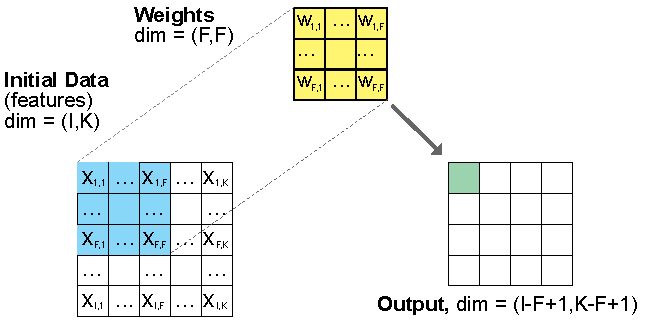
\includegraphics[width=0.7\linewidth]{files/cnn_scheme-8eb3e854b25a4e59e943b02e8593c6c9.pdf}

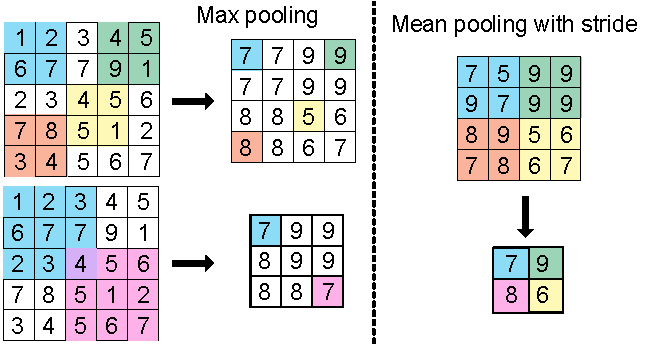
\includegraphics[width=0.7\linewidth]{files/cnn_pooling-05c87ceec9f840058ff626ad473215fa.pdf}

\subsubsection{Foundation models for tabular data}\label{foundation-tabular}

\paragraph{Presentation}

Foundation models pretrain a single large network once, often on synthetic data, and then adapt to a brand new task with no further gradient updates. This paradigm is well known for text and images and has recently reached tabular data. A pretrained transformer reads the whole training table as context and the test rows as a query, then returns predictions in one forward pass. There is no loss to minimize and no hyperparameter to tune at deployment time.

\cite{grinsztajn2022why} show that tree based models still beat plain deep networks on typical tabular data. This finding motivates a dedicated pretrained architecture rather than a generic network trained from scratch. \cite{hollmann2025accurate} introduce TabPFN, a transformer pretrained on millions of synthetic datasets that matches or beats tuned gradient boosting on small tables. \cite{qu2025tabicl} extend the idea with TabICL, a model built by the Inria team behind scikit learn, which scales in context learning to much larger tables through a two stage column then row attention mechanism.

For factor investing, this paradigm is appealing. Each rebalancing date can be treated as a small fresh dataset. The model reads the past cross section as context and predicts the next one, with no retraining between dates. Below, we illustrate this idea with TabICL. We pick this library because it installs with one pip command, downloads open weights with no license step, and handles regression directly.

The exercise below is a genuine out of sample test. For each test month $t$, the model is fit only on the single prior month and then applied to month $t$ features. Recall that in this book, \texttt{R1M} is dated at $t$ but stores the forward return realised between $t$ and $t+1$. So the model never sees the outcome it is scored on. We report two metrics. The first is the \textbf{information coefficient}, the cross sectional correlation between predicted and realised \texttt{R1M}. The second is the \textbf{long short decile Sharpe ratio}: each month we go long the top decile of predictions and short the bottom decile, and we annualise the mean and standard deviation of these twelve monthly spread returns.

\paragraph{Code and results}

\begin{verbatim}
import time
from sklearn.preprocessing import StandardScaler
from sklearn.linear_model import Ridge
from tabicl import TabICLRegressor

dates_sorted = sorted(data_ml_clean['date'].unique())
test_dates = dates_sorted[-13:-1]   # 12 rolling rebalancing dates

records = []
t0 = time.time()
for td in test_dates:
    idx = dates_sorted.index(td)
    train_date = dates_sorted[idx - 1]              # the single month strictly before td
    assert train_date < td                           # no look ahead: train date precedes test date

    Xtr = data_ml_clean.loc[data_ml_clean['date'] == train_date, features_short].values
    ytr = data_ml_clean.loc[data_ml_clean['date'] == train_date, 'R1M'].values
    Xte = data_ml_clean.loc[data_ml_clean['date'] == td, features_short].values
    yte = data_ml_clean.loc[data_ml_clean['date'] == td, 'R1M'].values   # forward return, unknown at td

    sc = StandardScaler().fit(Xtr)
    Xtr_s, Xte_s = sc.transform(Xtr), sc.transform(Xte)

    tab_mod = TabICLRegressor().fit(Xtr_s, ytr)
    pred_tab = tab_mod.predict(Xte_s)                # built only from Xte, the info available at td

    ridge_mod = Ridge(alpha=1.0).fit(Xtr_s, ytr)
    pred_ridge = ridge_mod.predict(Xte_s)

    q10t, q90t = np.percentile(pred_tab, [10, 90])
    q10r, q90r = np.percentile(pred_ridge, [10, 90])

    records.append({
        'date': td, 'train_date': train_date,
        'ic_tab': np.corrcoef(pred_tab, yte)[0, 1],
        'ic_ridge': np.corrcoef(pred_ridge, yte)[0, 1],
        'ls_tab': yte[pred_tab >= q90t].mean() - yte[pred_tab <= q10t].mean(),
        'ls_ridge': yte[pred_ridge >= q90r].mean() - yte[pred_ridge <= q10r].mean(),
    })

elapsed = time.time() - t0
res = pd.DataFrame(records)

# mean, std and Sharpe are reported separately so the computation is checkable
mu_tab, sd_tab = res['ls_tab'].mean(), res['ls_tab'].std()
mu_ridge, sd_ridge = res['ls_ridge'].mean(), res['ls_ridge'].std()
sharpe_tab = mu_tab / sd_tab * np.sqrt(12)
sharpe_ridge = mu_ridge / sd_ridge * np.sqrt(12)

print(f"Rebalancing dates covered   : {len(test_dates)}")
print(f"Total wall time             : {elapsed:.1f} seconds")
print(f"Train date always before test date : {(res['train_date'] < res['date']).all()}")
print()
print("Information coefficient (corr. between prediction and realised forward R1M):")
print(f"  TabICL : {res['ic_tab'].mean():.4f}")
print(f"  Ridge  : {res['ic_ridge'].mean():.4f}")
print()
print("Long short decile portfolio, monthly spread return statistics (12 test months):")
print(f"  TabICL : mean={mu_tab:.4f}  std={sd_tab:.4f}  annualised Sharpe={sharpe_tab:.2f}")
print(f"  Ridge  : mean={mu_ridge:.4f}  std={sd_ridge:.4f}  annualised Sharpe={sharpe_ridge:.2f}")
\end{verbatim}

\begin{verbatim}
Rebalancing dates covered   : 12
Total wall time             : 53.1 seconds
Train date always before test date : True

Information coefficient (corr. between prediction and realised forward R1M):
  TabICL : -0.0090
  Ridge  : -0.0144

Long short decile portfolio, monthly spread return statistics (12 test months):
  TabICL : mean=-0.0092  std=0.0730  annualised Sharpe=-0.44
  Ridge  : mean=-0.0076  std=0.0693  annualised Sharpe=-0.38
\end{verbatim}

The check above confirms every fold trains strictly before it tests, so the numbers are out of sample by construction, not synchronous. Both Sharpe ratios are negative. This is worth underlining: a negative Sharpe means the long short strategy loses money on average over these twelve months, for both models. This illustrates one of the recurring messages of this book: machine learning in finance is not a plug and play exercise. A powerful state-of-the-art model does not automatically produce good returns. Turning a model into profits takes careful feature engineering, thoughtful validation, sensible portfolio construction, and plain domain expertise. None of that is present in the minimal setup used here. Note also that TabICL involves some internal randomness, so rerunning this cell can shift the numbers slightly without changing the overall picture.

\subsubsection{Coding exercises}

\begin{enumerate}
\item Code the autoencoder model described in \cite{gu2019autoencoder} using the functional API.
\item Demonstrate the universal approximation of simple NNs by approximating sin(x) over [0,6] with 16 and then 128 units.
\end{enumerate}